\documentclass{assignment}
\usepackage{wrapfig}
\usepackage{array}
\usepackage[export]{adjustbox}
\usepackage{multirow}
% \usepackage[demo]{graphicx}

\begin{document}

\assignmentTitle{Irene Ferrari 10699084}{Silvia Alessandra Michela Fiecchi 10702310}
{Pedro Guimarães Marcal 10855687}{Roberto Reggiani 10539876}{Jacopo Stringara 10687726}
{assets/logo.png}{Computational Finance - Asset Allocation}{Exam: version C} 
{Lecturers: D.Marazzina, G.Angelini, A.Y. 2023/2024}

\section*{Introduction and Objectives}
In the context of the course of Computational Finance module of Asset Allocation, this report shows
our development and analysis following the theoretical knowledge received in lectures and its
purpose applied to the given financial data. As it will be explained in the following, the data
consists of daily prices of 100 US companies as well as their Market Capitalization and Sectors. \\
Throughout this report we will compare and analyze different portfolios and allocation strategies.

\section*{Data overview: S\&P100 indices}
The investment universe provided for portfolio construction consists of the assets included in the
S\&P 100 stock market index. A preliminary empirical analysis was needed in order to understand
which results could be reasonably expected.\\
As part of the S\&P Dow Jones Indices family, the S\&P 100 operates as a subset of the broader S\&P
500, encompassing the 500 largest publicly traded U.S. companies, including various sectors
according to which the assets in the data set were divided. The 100 selected companies embodied in
the S\&P 100 index, represent the largest and most established companies listed on both the NYSE
and NASDAQ and they typically represent leaders within their respective industries and are
classified as large-cap, denoting their substantial market capitalization.\\
Henceforth, investors commonly utilize the S\&P 100 as a benchmark to assess portfolio performance
or make comparisons with alternative investments. Historically, the S\&P 100 has mirrored the
profitability of major, well-established corporations, thus we expect positive long-term returns.
As regards volatility considerations, generally large-cap stocks, as typified by the S\&P 100, are
characterized by lower volatility compared to their smaller-cap counterparts, owing to greater
stability and resilience.  Nevertheless, fluctuations in volatility levels can occur, particularly
during periods of economic uncertainty or market turbulence.

\section*{Part A}
For the first part of the analysis, prices for the dates ranging from 11/05/2021 to 11/05/2022 were
considered. We assumed throughout the whole report that the risk free rate is null. Consistent with
what was done for the analysis of the securities under study, a critical analysis of the market
situation during this period was conducted.\\
Despite the momentum provided by the global economic growth rebound following the reopening of
economic activities stalled by the Sars Covid 19 pandemic, the initially considered increase in
inflation, deemed by Federal Reserve Chairman Jerome Powell as a cyclical factor, translated into
the abandonment of expansive monetary policies and a shift towards restrictive ones in early 2022.
The FED embarked on a path of monetary policy normalization, with a tapering phase starting in
November 2021 and the initiation of interest rate hikes, settling between 5.25\%-5.50\% in the
United States. Stock markets in 2022 experienced a general decline, with the S\&P 500 closing with
a -20\% decrease.\\
Hence, in our analysis we now expect all portfolios to have negative or low return rates and in
general to perform rather poorly in the given period due to the overwhelming market trends at work.
As a matter of fact, we see in the following picture the price of the S\&P 100 in the considered
time range and, as expected, it shows the aforementioned behaviour.
\begin{center}
    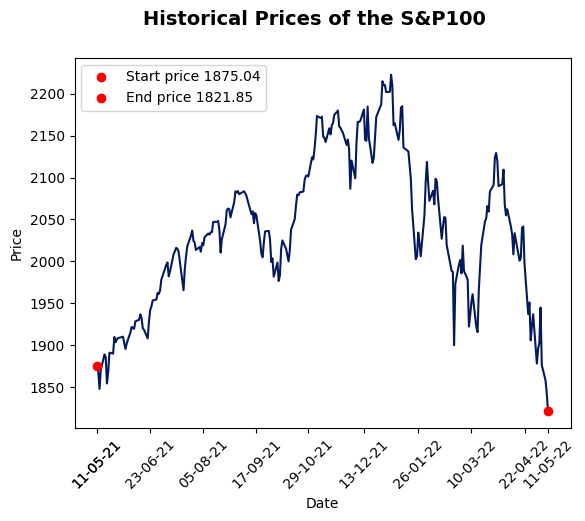
\includegraphics[height=7cm]{assets/Unknown-12.png}
\end{center}

\subsection*{Exercise 1}
Firstly, we were tasked with computing the efficient frontier under the standard constraints, as
introduced by Nobel Laureate Harry Markowitz in 1952. The standard constraints are: 
\[
    \sum_{i}^{N}{w_{i}} = 1 \quad and \quad
    0\leq w_i \leq 1 ,\quad  \forall i\in \left [ 1,..,N \right ]  
\]
where N represents the total number of assets.\\ 
Following the necessary data type transformations, we opted to use the existing \textbf{Matlab}
functions provided by Financial Toolbox, since they performed best with respect to the other
possible approaches.

\begin{tabular}{c m{0.43\textwidth}}
    % first column is the graph
    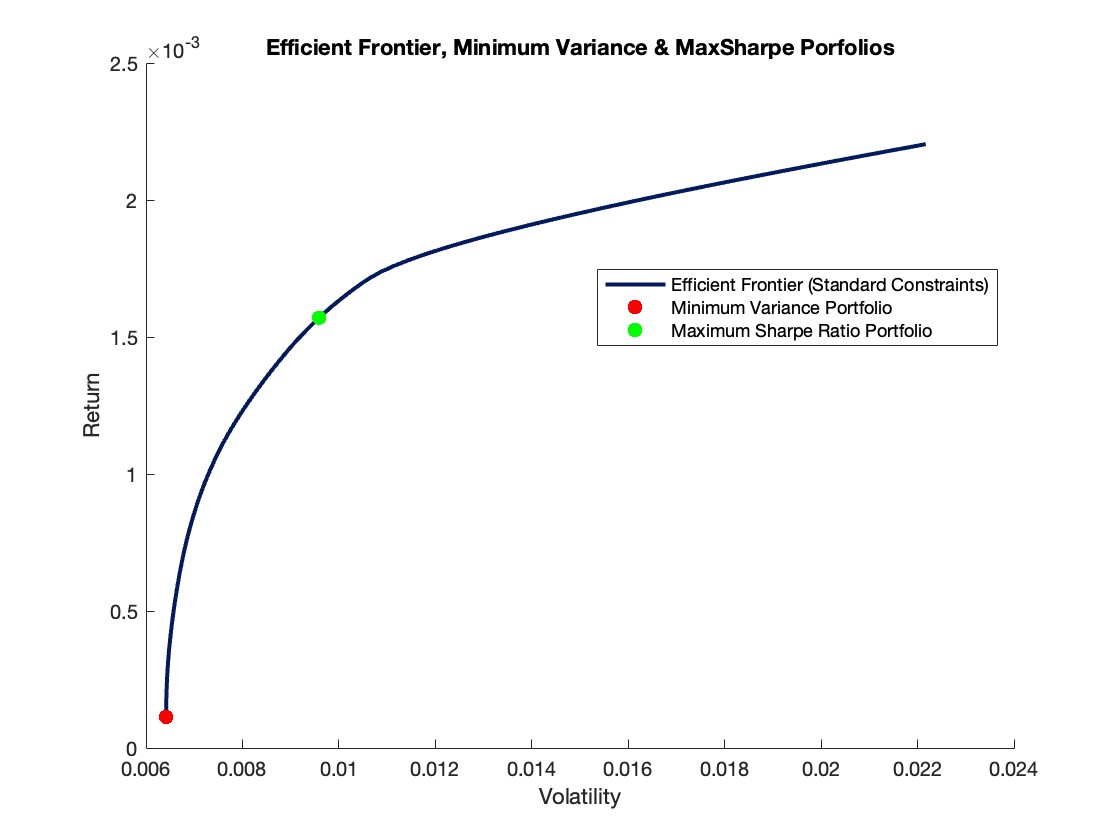
\includegraphics[width=0.50\textwidth, valign=c]{assets/Plot_1.jpg}
    &
    On the left, we present the resulting \textbf{Efficient Frontier}. The chart allows to observe
    how portfolios are positioned along the efficient branch of the portfolio frontier due to a
    successful optimization of the return versus risk paradigm. We expect that optional portfolios
    comprising the efficient frontier exhibit a higher degree of diversification compared to
    sub-optimal portfolios. Overall, portfolio returns are moderate with low values of volatility. 
\end{tabular}
\\
We then proceeded to compute the Minimum Variance (\textbf{PORTFOLIO A}) and Maximum Sharpe Ratio
(\textbf{PORTFOLIO B}) Portfolios.

\begin{center}
    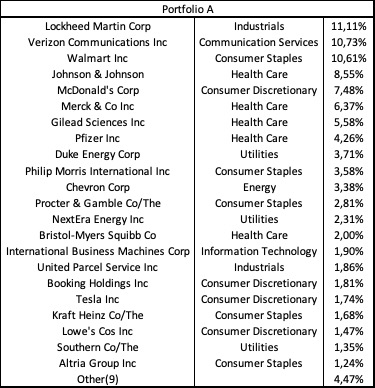
\includegraphics[height=6cm]
    {assets/Port_A.jpg}
    \quad
    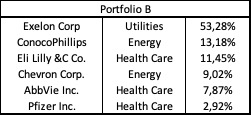
\includegraphics[height=2cm]
    {assets/Port_B.jpg}
\end{center}
\textit{(For readability reasons, we put under "Other" all the assets with weight lower than 1\%)}
\\\\
\textbf{Portfolio A}: ExpLogRet = 1.1352e-4, Vol = 0.0064\\
\textbf{Portfolio B}: ExpLogRet = 1.5704e-3, Vol = 0.0096
\\\\
Comparing the portfolios, the Minimum Variance Portfolio is the most diversified, as a consequence
of minimizing the variance. On the other hand, the Maximum Sharpe Ratio portfolio is concentrated
in Exelon Corp, which is the American leading energy provider, reflecting the Global Energy Crisis
in 2021, and the war in Ukraine in February 2022.\\
The Maximum Sharpe Ratio portfolio will serve as our starting point, as according to Markowitz's
theory, it indicates the optimal balance between risk and return. In fact, it represents the point
with the steepest slope on the frontier.\\
Both portfolios have limited returns, which can be attributed to the socio-economic conditions of
the historical period. However, increasing the variance by 0.0032, we obtain an expected return 10
times higher, confirming once again the better performance of the Maximum Sharpe Ratio Portfolio.

\subsection*{Exercise 2}
We here introduced additional constraints representing potential investment choices.
For better performance reasons, we opted again for the built-in \textbf{Matlab} functions and
maintained standard constraints, to be now enriched with the following ones.

\begin{align*}
    \sum_{i}^{CD}{w_{i}} > 0.15 \quad , \quad 
    \sum_{i}^{I}{w_{i}} < 0.05 \quad , \quad
    0\leq w_i \leq 1 ,\quad  \forall i\in \left [ 1,..,N \right ]  
\end{align*}
The first constraint imposes that the overall exposure of the companies belonging to the sector
"Consumer Discretionary" (here CD) has to be greater than 15\%, while the second one that the
overall exposure of the companies belonging to the sector "Industrials" (here I) has to be less
than 5\%.
Furthermore, the companies in the Energy, Materials, Real Estate and Utilities were not considered
as their sectors contain less than five companies in our data set. 
We, then, proceeded to compute the Minimum Variance Portfolio and Maximum Sharpe Ratio Portfolio
under these new hypotesis.

\begin{tabular}{c m{0.43\textwidth}}
    % first column is the graph
    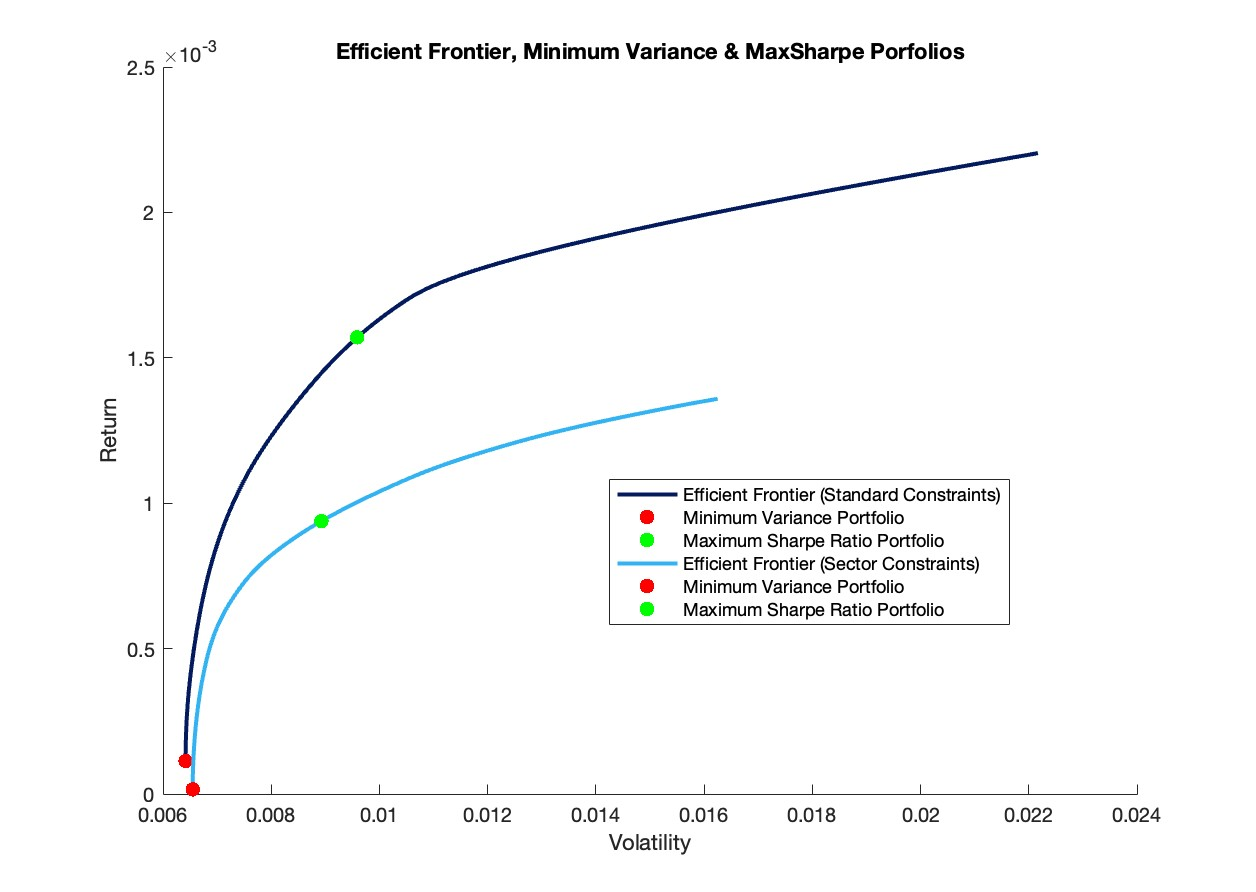
\includegraphics[width=0.50\textwidth, valign=c]{assets/Plot_2.jpg}
    &
    On the left, it is possible to compare the efficient frontiers constructed with and without
    sector constraints. We observed that the new frontier is situated within a narrower range of
    volatility and, concurrently, exhibits lower returns. In addition, considering the return
    fixed, we have a much higher value of volatility. This can be explained by the fact that adding
    the constraints, we cannot diversify as much as before.
\end{tabular}
We then proceeded to compute the Minimum Variance (\textbf{PORTFOLIO C}) and the Maximum Sharpe
Ratio (\textbf{PORTFOLIO D}) Portfolios on this new constrained frontier.
\begin{center}
    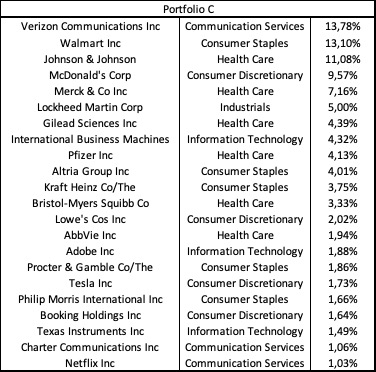
\includegraphics[height=6cm]
    {assets/Port_C.jpg}
    \quad
    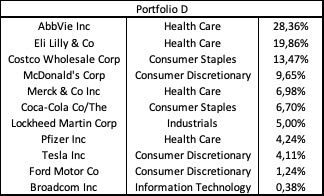
\includegraphics[height=3cm]
    {assets/Port_D.jpg}
\end{center}
\textit{(For readability reasons, we omitted all the assets with weight lower than 1\%)}\\\\
\textbf{Portfolio C}: ExpLogRet = 1.583e-5, Vol = 0.0065\\
\textbf{Portfolio D}: ExpLogRet = 9.384e-4, Vol = 0.0089\\
\\
The introduction of the additional constraints led to a decrease in expected returns in both
corresponding portfolios. 
In particular, considering the Minimum Variance Portfolio, we observed a decrease by a factor of 10
in the expected return. On the other hand, the decrease in the Max Sharpe Ratio Portfolio's
expected return was smaller. 
Therefore, while the distance between the volatilities of the two portfolios remains about the same
as before adding the constraints, the distance between the expected returns increases by almost a
factor of 10. 
Overall, we can see a noticeable and varied increase in the number of stocks in the "Consumer
Discretionary" sector, as expected, while in Portfolio C the "Industrials" sector is wholly
occupied by the Lockheed Martin Corp, following the introduction of the sector constraints.

\subsection*{Exercise 3}
Here we computed the frontiers from exercises 1 and 2 using a re-sampling method to obtain robust
frontiers for each of the set of constraints. It is well established that Frontier Resampling
effectively addresses specific limitations inherent to Mean-Variance Analysis, including the
management of non-normally distributed data and the incorporation of tail risk and extreme events.
Moreover, it can be extended to consider dynamic factors and changing market conditions over time,
allowing investors to build portfolios that adapt to evolving economic and market environments.\\\\
We opted for 50 different simulations, sampling the returns and multivariate normal variables and
constructing the efficient frontier as the mean of the simulated frontiers.\\
In accordance with the foregoing, it is possible to visually inspect the computed frontiers. 

\begin{center}
    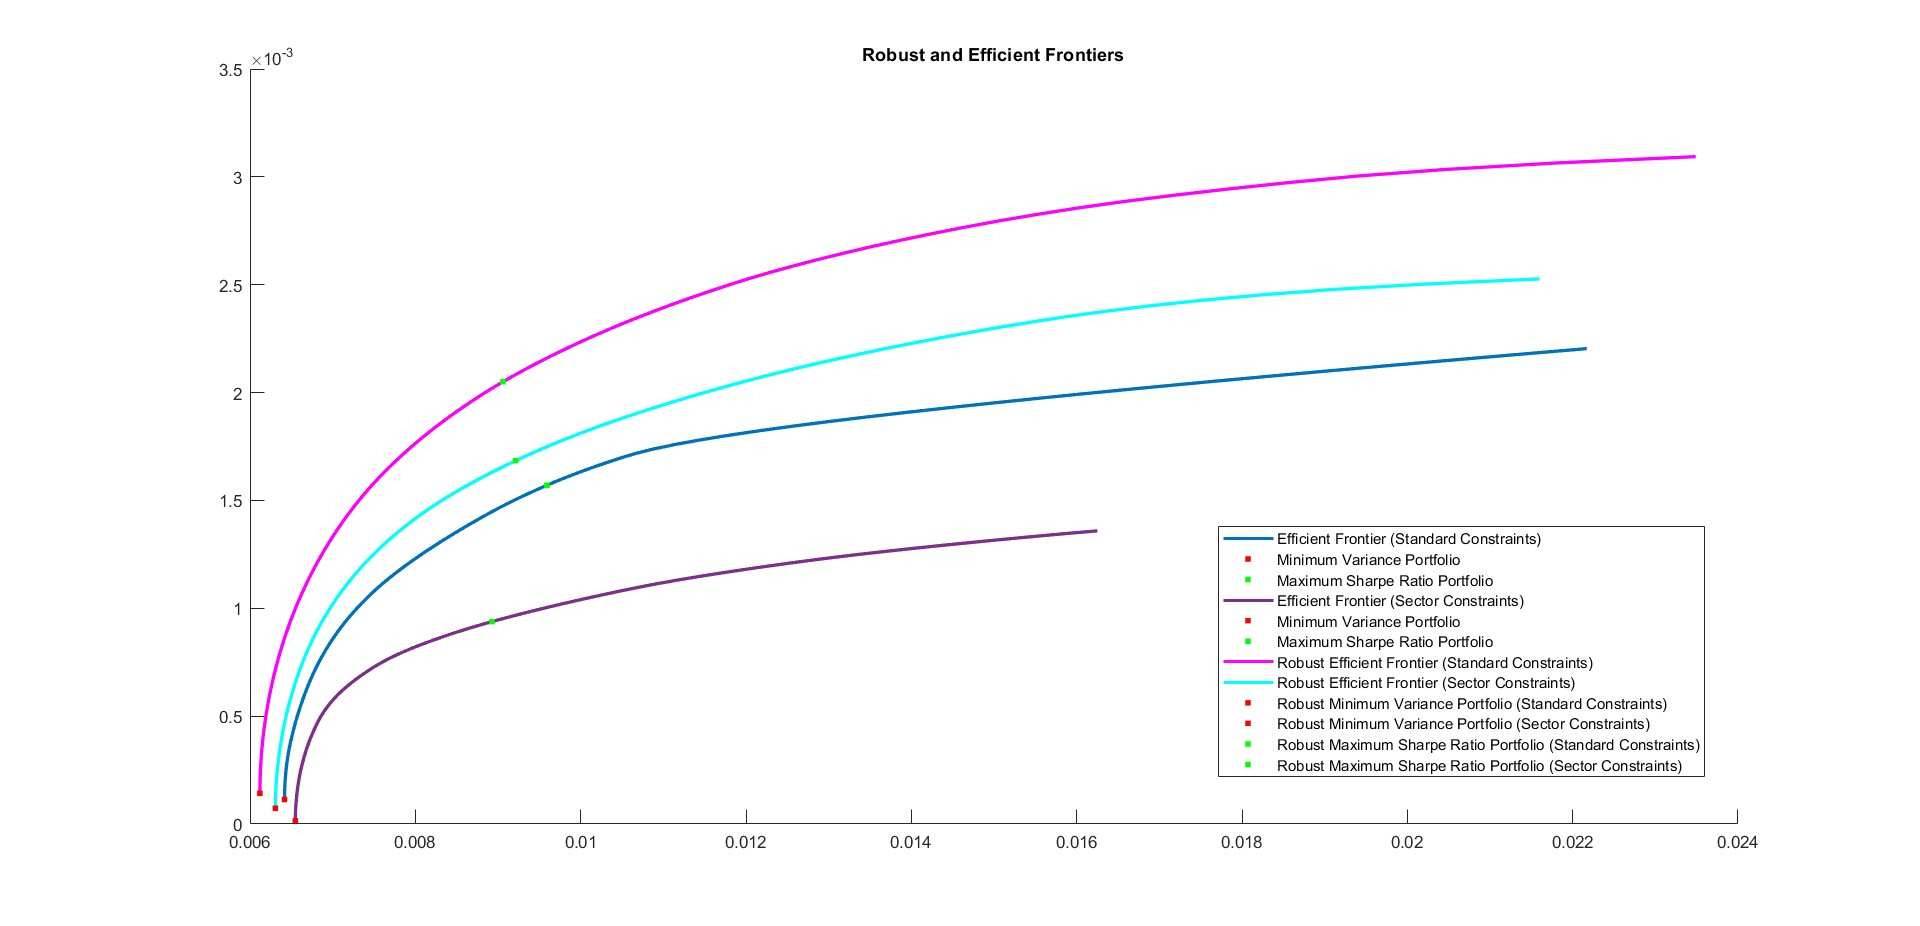
\includegraphics[height=6.5cm]{assets/Plot_3.jpg}
\end{center}
\bigskip
As expected from the general context, it is discernible that Robust Frontiers afford enhanced
diversification in the allocation, yielding higher returns while exhibiting a relatively stable
range of volatility. \\\\
Once again, we were interested in the Minimum Variance and Maximum Sharpe Ratio portfolios.\\
\textbf{Portfolio E} and \textbf{Portfolio G} were computed with standard constraints.

\begin{align*}
    \sum_{0}^{N}{w_{i}} = 1 \quad and \quad
    0\leq w_i \leq 1 ,\quad  \forall i\in \left [ 1,..,N \right ]  
\end{align*}


Obtaining the following assets weights: 
\begin{center}
    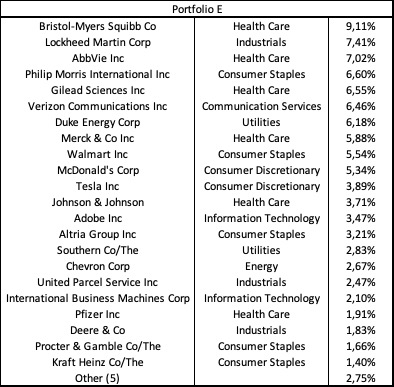
\includegraphics[height=6cm]
    {assets/Port_E.jpg}
    \quad
    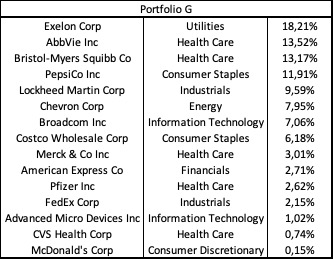
\includegraphics[height=4.5cm]
    {assets/Port_G.jpg}
\end{center}
\textit{(For readability reasons, we put under "Other" all the assets with weight lower than 1\%)}
\\\\
\textbf{Portfolio E}: ExpLogRet = 2.193e-4, Vol = 0.0067 \\
\textbf{Portfolio G}: ExpLogRet = 9.183e-4, Vol = 0.0075\\\\
\textbf{Portfolio F} and \textbf{Portfolio H} were computed incorporating sectoral constraints as
above. 

\begin{align*}
    \sum_{i}^{CD}{w_{i}} > 0.15 \quad , \quad 
    \sum_{i}^{I}{w_{i}} < 0.05 \quad , \quad
    0\leq w_i \leq 1 ,\quad  \forall i\in \left [ 1,..,N \right ]  
\end{align*}\\
We obtained the following Portfolios: 
\begin{center}
    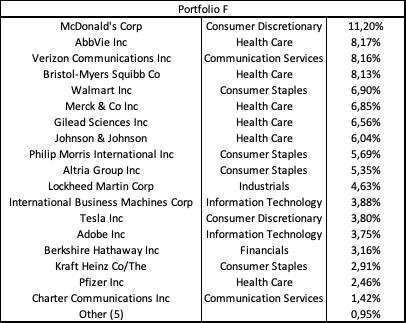
\includegraphics[height=6cm]
    {assets/Port_F.jpg}
    \quad
    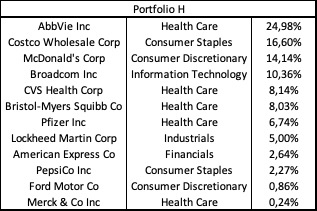
\includegraphics[height=4.5cm]
    {assets/Port_H.jpg}
\end{center}
\textit{(For readability reasons, we put under "Other" all the assets with weight lower than 1\%)}
\\\\
\textbf{Portfolio F}: ExpLogRet = 1.733e-4, Vol = 0.0067\\ 
\textbf{Portfolio H}: ExpLogRet = 7.602e-4, Vol = 0.0085\\\\
Once again, considering sectoral constraints determines a decrease in the return of the portfolios
under study, with a slightly lower volatility as well.


\subsection*{Exercise 4}
We undertook the computation of the portfolio frontier, under standard constraints, employing the
Black-Litterman model. This model facilitates the incorporation of the investor's views or beliefs
regarding expected returns. In fact, the standard mean-variance optimization relies exclusively on
historical data, which may result in suboptimal portfolios that do not reflect current market
conditions or investor expectations.\\
\\
\begin{tabular}{c m{0.46\textwidth}}
    % first column is the graph
    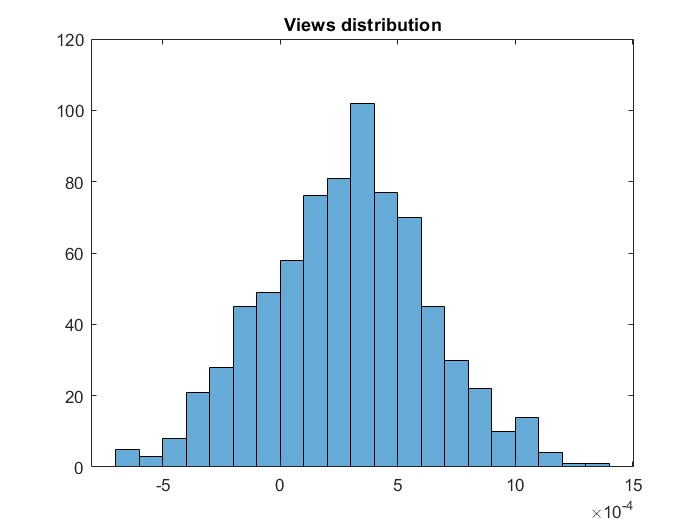
\includegraphics[width=0.50\textwidth, valign=c]{assets/Views_distr.jpg}
    &
    We imposed the desired conditions on "Consumer Staples" and "Healthcare" sectors annual returns
    (= 7\% and = 4\% respectively) and asked that companies belonging to the sector "Communication
    Services" outperform the companies belonging to the sector "Utilities" of 4\%. We can visualize
    views distributions on the left. 
\end{tabular} 
\\
In this section, we assumed the investor exhibited a moderate risk profile, setting the risk
aversion coefficient to 1.2. We computed the efficient frontier.

\begin{center}
    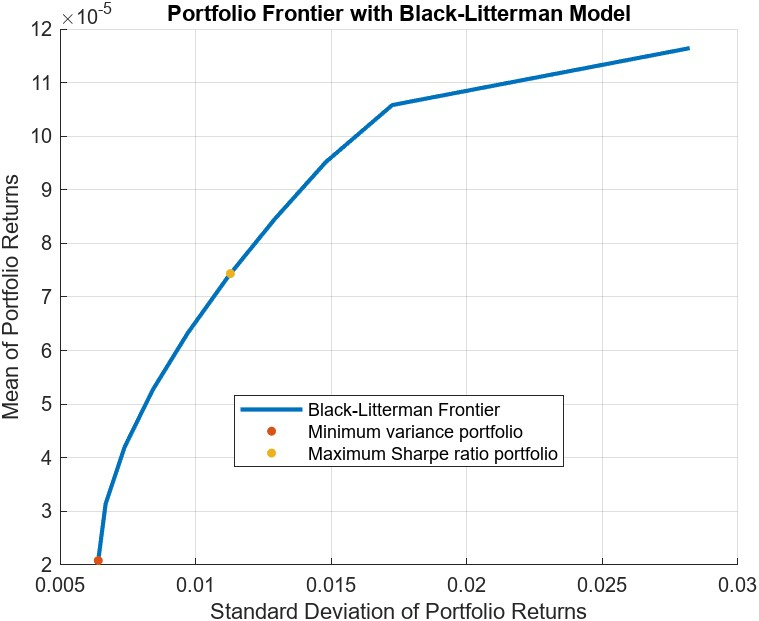
\includegraphics[height=8cm]
    {assets/frontierBL.jpg}
\end{center}
The resulting frontier, shown above, computed under standard constraints, is more adaptable to the
individual preferences and market conditions. 
\\\\
We finally computed the Minimum Variance (\textbf{PORTFOLIO I}) and the Maximum Sharpe Ratio
(\textbf{PORTFOLIO L}) portfolios. 

\begin{center}
    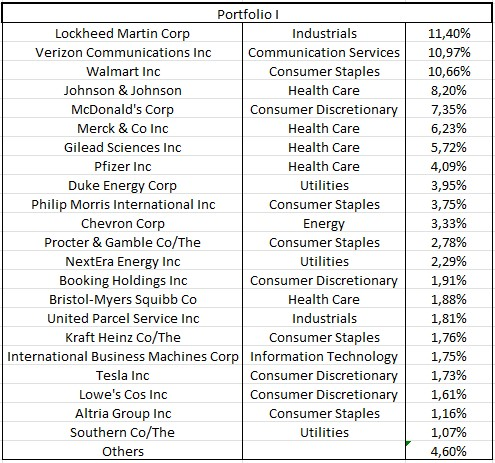
\includegraphics[height=7cm]
    {assets/Port_I.jpg}
    \quad
    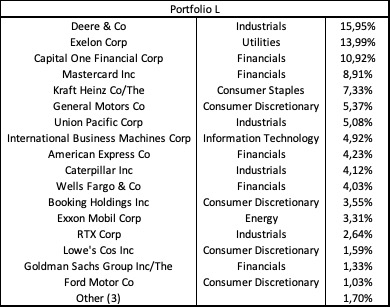
\includegraphics[height=5.5cm]
    {assets/Port_L.jpg} 
\end{center}
\textit{(For readability reasons, we put under "Other" all the assets with weight lower than 1\%)}
\\\\
\textbf{Portfolio I}: ExpRet = 2.0808e-5, Vol = 0.0064\\
\textbf{Portfolio L}: ExpRet = 7.43641e-5, Vol = 0.0113\\\\
As expected from the theory behind Black-Litterman Model, both the Mean Variance Portfolio and the
Maximum Sharpe Ratio Portfolio are more diversified than before and in line with the investor's
views. 

\subsection*{Exercise 5}
In this section we operated under the standard constraints:
\begin{align*}
    \sum_i^N w_{i} = 1 \quad and \quad
    0\leq w_i \leq 1 ,\quad  \forall i\in \left [ 1,..,N \right ]  
\end{align*}
Furthermore we also considered the following:
\begin{align*}
    0.001 \leq w_i \leq 0.02 \quad i \in \text{ Financial sector} \\
    0.005 \leq w_i \leq 0.01 \quad i \in \text{ Industrial sector}
\end{align*}
Then we computed, using the \textit{fmincon} function in \textbf{Matlab}, the Maximum Diversified Portfolio (\textbf{PORTFOLIO M}) and the Maximum Entropy portfolio (\textbf{PORTFOLIO N}). \\
These portfolios ignore all assumptions on expected returns, and instead focus on the diversification and mitigation of risk, using two different measures for diversification.\\
Portfolio M maximizes the diversification ratio metric, which measures the effectiveness of diversifying investments in the portfolio, while Portfolio N maximizes the entropy as a function of the asset volatilities.\\
The composition for portfolio M and N can be found below:

\begin{center}
    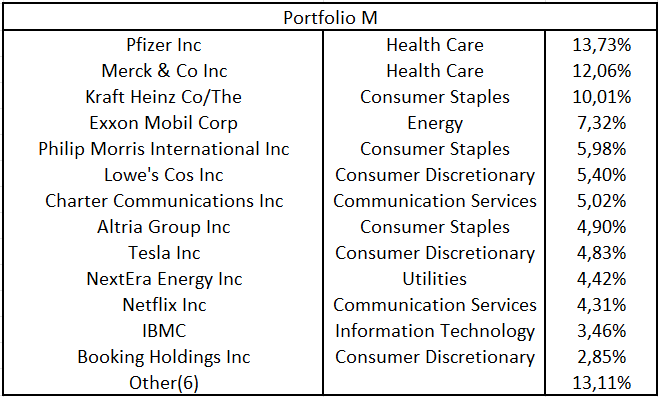
\includegraphics[height=4cm]
    {assets/Port_M.png} 
    \quad
    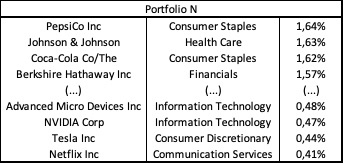
\includegraphics[height=4cm]
    {assets/Port_N.jpg} 
\end{center}
\textit{(For readability reasons, we put under "Other" all the assets with weight lower than 1\%)}\\\\
\textbf{Portfolio M}: ExpLogRet = -7.5927e-6, Vol = 0.0076, Diversification Ratio = 2.3653, Entropy = 2.2684\\
\textbf{Portfolio N}: ExpLogRet = -1.7194e-4, Vol = 0.0087, Diversification Ratio = 1.8063, Entropy = 4.5748\\\\
In this case, we obtain for both portfolios a negative Expected Logarithmic Return, which can be justified by the fact that, as reported above, both portfolios aim just to decrease the risk, and that the Expected Logarithmic Returns of the assets are mostly negative, as observed in our preamble. Likewise the Equally Weighted portfolio has a negative Expected Logarithmic Return, which is probably related to the bearish behaviour of the market.

\subsection*{Exercise 6}
In this section, we employed Principal Component Analysis to limit ourselves to 10 different factors.
These factors can be interpreted to be the 10 most influential portfolios in the market, which drive its evolution.\\
We then maximized the expected return under standard constraints and a target volatility $\sigma_{tgt} = 0.007$ using the \textit{fmincon} function.\\
The PCA methodology yielded the following explained variance graphs:
\begin{center}
    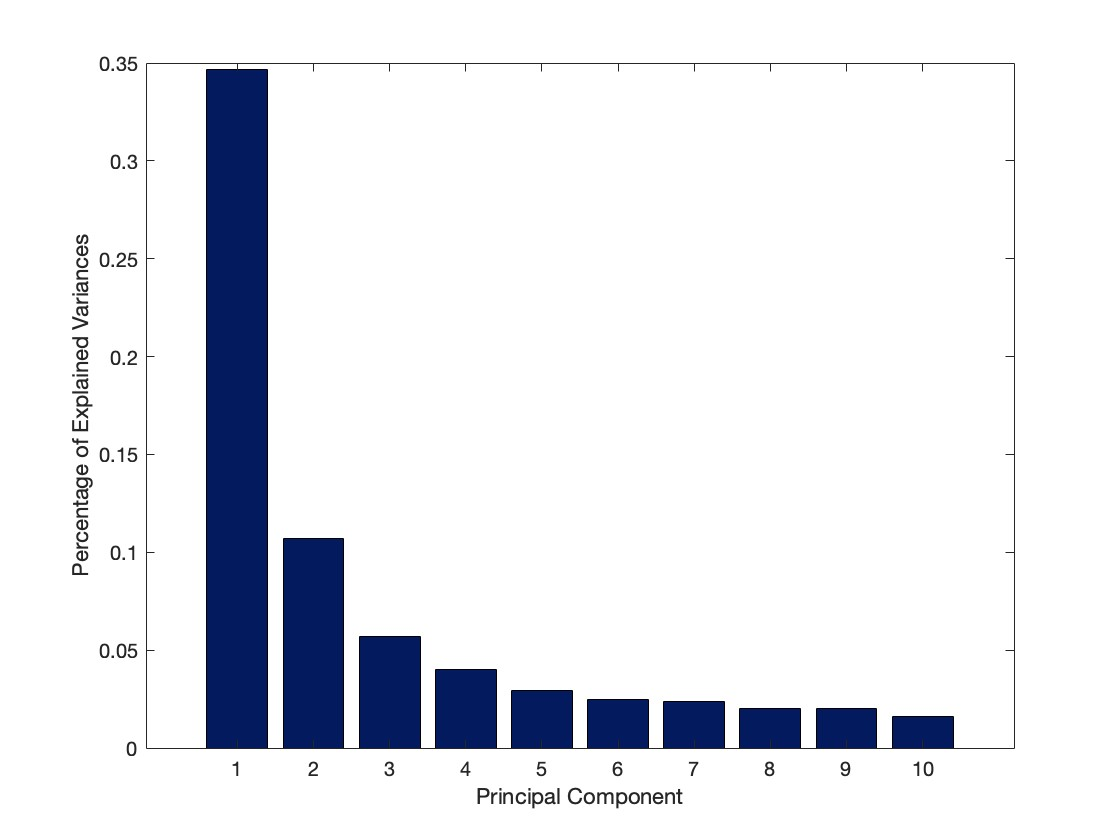
\includegraphics[width=0.45\textwidth]{assets/Hist2.jpg}
    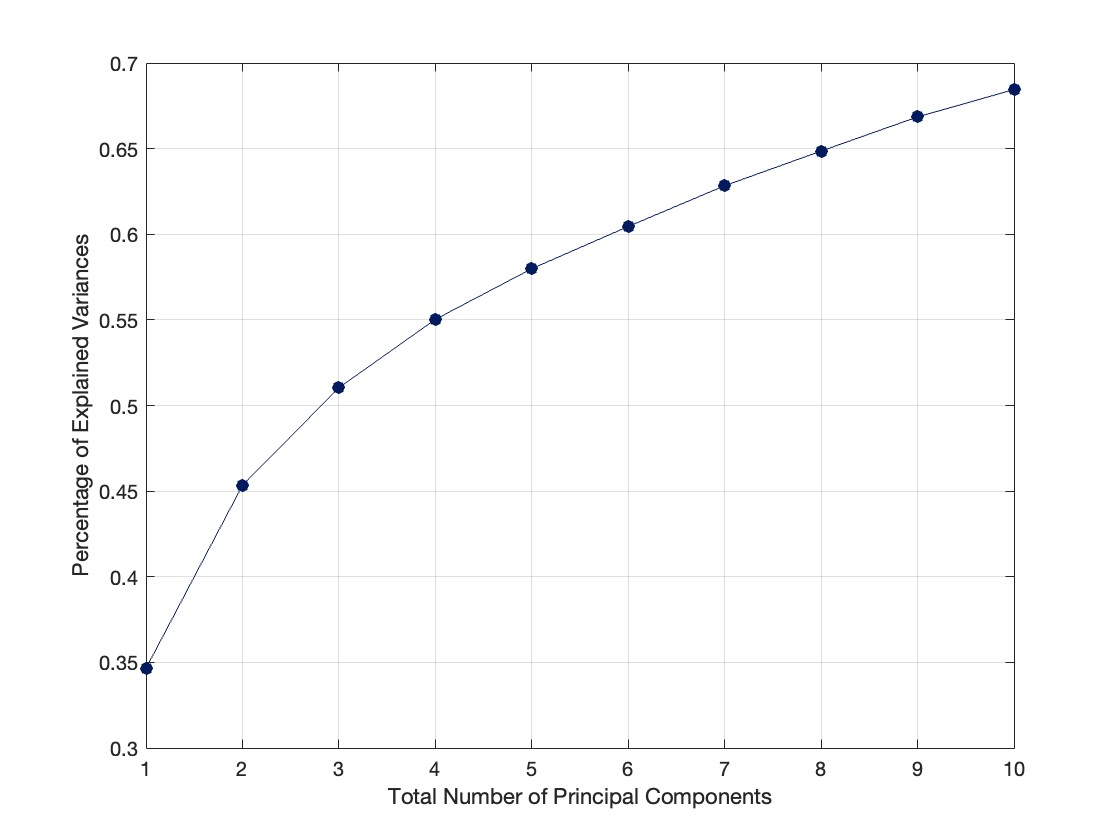
\includegraphics[width=0.45\textwidth]{assets/Plot_7.jpg}
\end{center}
As we can see, the first influencial portfolio explains 35\% of market variance, and all 10 most influential components explain almost 70\% of market variance.
We then computed the Portfolio that maximizes the expected return (\textbf{PORTFOLIO P}) in this framework, obtaining:
\begin{center}
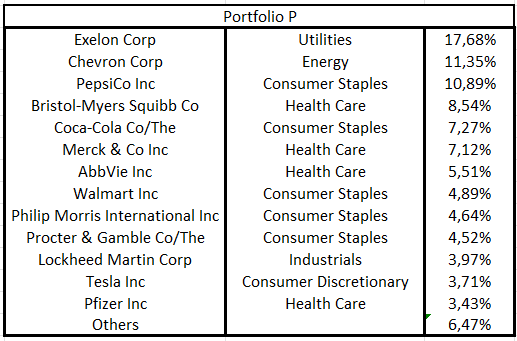
\includegraphics[width=0.50\textwidth]{assets/Port_P.png}
\end{center}
\textit{(For readability reasons, we put under "Other" all the assets with weight lower than 1\%)}\\\\
\textbf{Portfolio P}: ExpLogRet = 8.740e-4, Vol = 0.007\\\\
The PCA-driven allocation highlights the diversification benefits achieved by capturing the principal components of the asset returns. The portfolio sheds light  on the dominant factors influencing the portfolio's performance, increasing their weights. 

\subsection*{Exercise 7}
In this section, we employed a modified version of the Sharpe Ratio. Here we use the Expected Shortfall (calculated under the assumption that the data is Normal, which seems to be valid plotting the qq-plot of the logarithmic return of each asset, see picture below), as a  way to measure risk instead of the classical approach of using volatility.
\begin{center}
    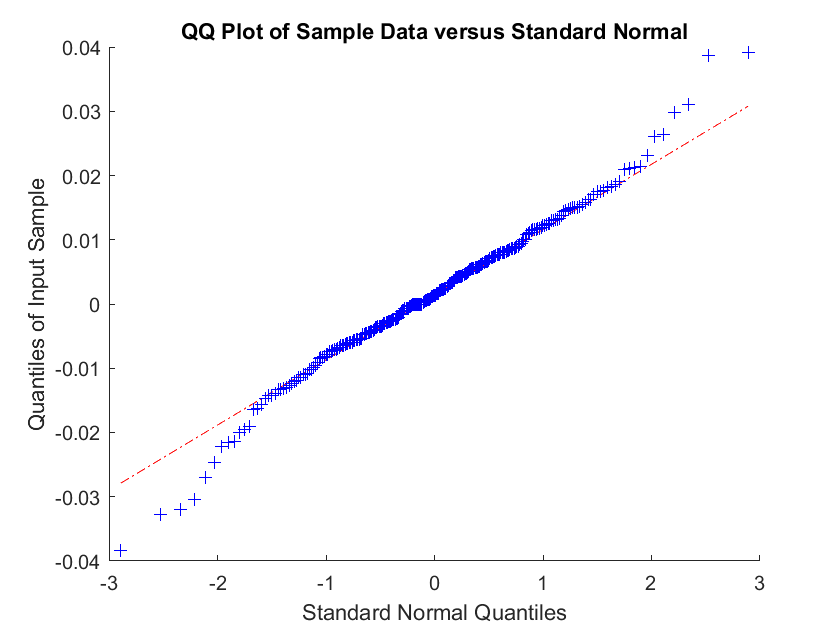
\includegraphics[width=0.50\textwidth]{assets/qqplot.png}
\end{center}
\bigskip
\[
    Sharpe_{modified} = \frac{\mu_{pf}}{ES_{pf}  } \text{ with }  ES_{pf} = \mu_{pf} + \sigma_{pf} \cdot
    \frac{\phi(\Phi^{-1}(1-p))}{p}
\]
\medskip \\
where $\phi$ and $\Phi$ are the standard normal pdf and cdf. Furthermore, we assumed $p=0.05$ since this is one of the most common values for $p$ in the industry.\\
At this point, we again employed the help of the \textit{fmincon} function to compute the Maximum Modified Sharpe Ratio portfolio (\textbf{PORTFOLIO Q}), under standard constraints. This yielded the following portfolio values:

\begin{center}
    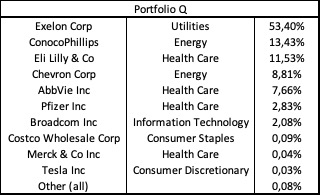
\includegraphics[width=0.5\textwidth]{assets/Port_Q.jpg}
\end{center}
\bigskip
\textbf{Portfolio Q}: ExpLogRet = 0.0016, Vol = 0.0096, Modified Sharpe Ratio = 0.0735

\subsection*{Discussion - Exercise 8}
In order to evaluate the performance and some characteristics of the computed portfolios we calculated the following parameters: Annualized Returns, Annualized Volatilities, Sharpe Ratio, Maximum Drawdown, Calmar Ratio and Diversification Ratio for each portfolio.
Above all we can notice how Calmar Ratio and Sharpe Ratio tend to be correlated while the diversification ratio and the Maximum Drawdown are not as strongly correlated.


\begin{center}
    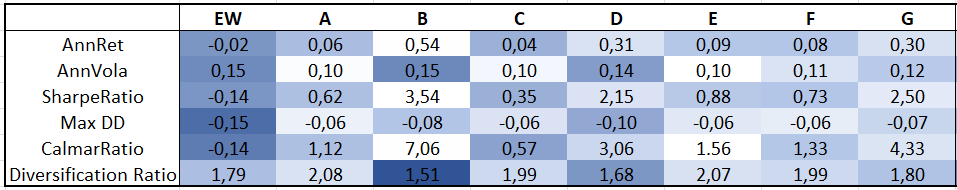
\includegraphics[height=2.5cm]
    {assets/Blue1.png}
\end{center}

\begin{center}
    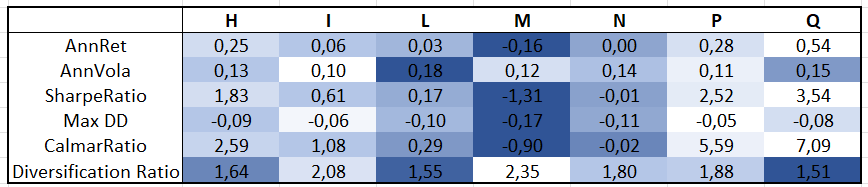
\includegraphics[height=2.5cm]
    {assets/Blue2.png}
\end{center}


Having the Equally weighted portfolio as a reference we do not expect extreme returns for most of the computed portfolios as the average return of the equities in the time period, 11/05/2021 to 11/05/2022, was negative. Despite this, our portfolios that maximize the Sharpe Ratio have the best returns. Which was expected since the metrics used for building the portfolios are based in the performance/risk behaviour of our equities in the same time period.
Once again, using the Equally Weighted portfolio as a starting point we can see that all of the computed portfolios have comparable annualized volatility.
Specifically from the metrics we can appreciate how the different algorithms of optimization work. The portfolios which try to maximize the Sharpe Ratio (B,D,G,H) do so at the cost of having a higher variance of their counter part with the same constraints and algorithm (A,C,E,F).
It's interesting to see how the Portfolio M, that maximizes the diversification ratio, has as a result the worst Sharpe Ratio and consequently one of the worst equities. On the opposite both Portfolio B and the Expected Shortfall-modified Sharpe Ratio portfolio, that have the worst diversification ratio, have the highest equity.
Indeed, there is a striking similarity between portfolio B and Q on the values of all metrics. Due to this we noticed that the two portfolios, despite the use of modified Sharpe Ratio give almost the same weights. This is probably due to the presence of a handfull of very high performance stocks, such as Exelon Corp, which have a very high yield and relatively low volatility.
The Maximum Drawdown of the portfolios is of course correlated to their annualized volatility and diversification. This is due to the fact that it is a measure related to the difference between peaks and troughs which is in itself related to the variance of the price process of the equities in the portfolio.
%se si vuole mettere differenza quadratica tra i due vettori dei pesi come formula con il risultato. 

The most interesting Portfolios for our analysis are the following: Maximum Sharpe standard constraints (D), Principal Component Analysis (P) Expected Shortfall-modified Sharpe Ratio (Q) and Maximum Diversification (M). 
Here we can see the Equity of these 4 portfolios, compared to the one of the Equally Weighted Portfolio, used as benchmark.

\begin{center}
    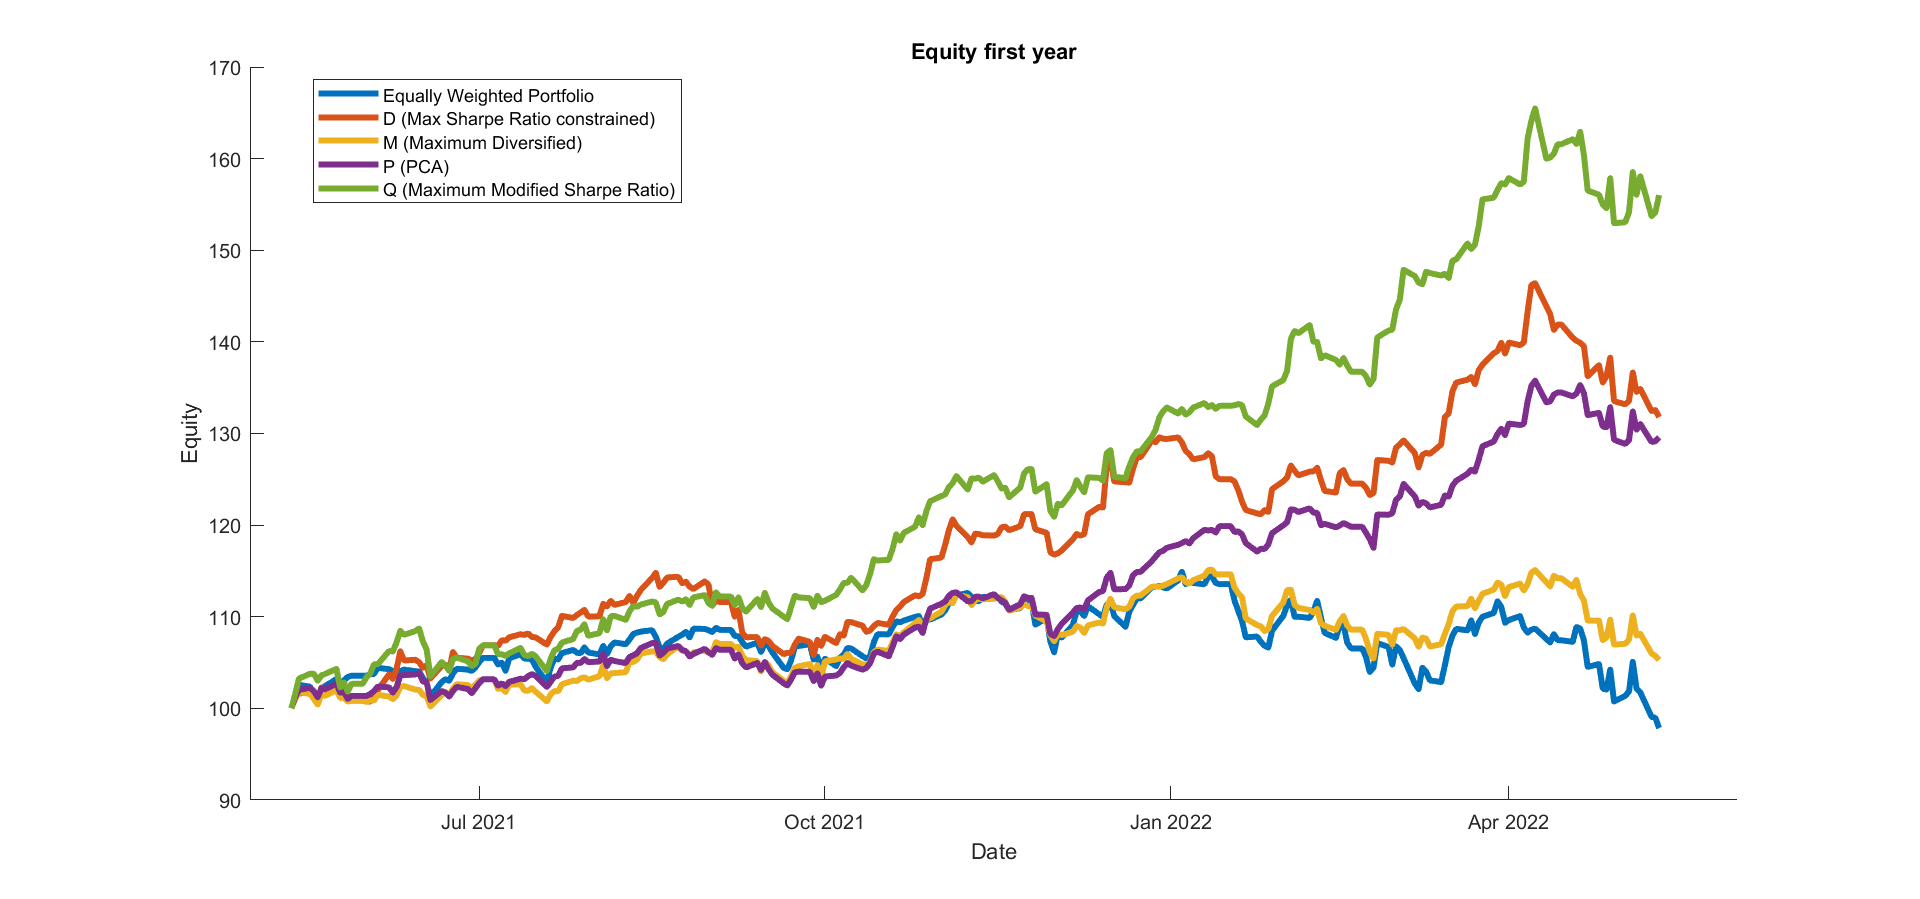
\includegraphics[height=7cm]
    {assets/Equity1.png}
\end{center}

\section*{Part B}

\subsection*{Initial Considerations}
When evaluating the performance of previous portfolios and comparing their characteristics, we overlooked a crucial economic parameter and a key feature of the considered equities.\\
Firstly, when calculating the Sharpe Ratio, we traditionally factor in the risk-free rate. In the given period of 2021-2022, this rate could be deemed close to zero, given the historically low interest rates. However, in the aftermath of the pandemic and the subsequent inflationary pressures, central banks globally found themselves compelled to raise interest rates, impacting the entire financial system. It is worth noting that we can visually represent the FED interest rates from May 2021 to May 2023.

\begin{center}
    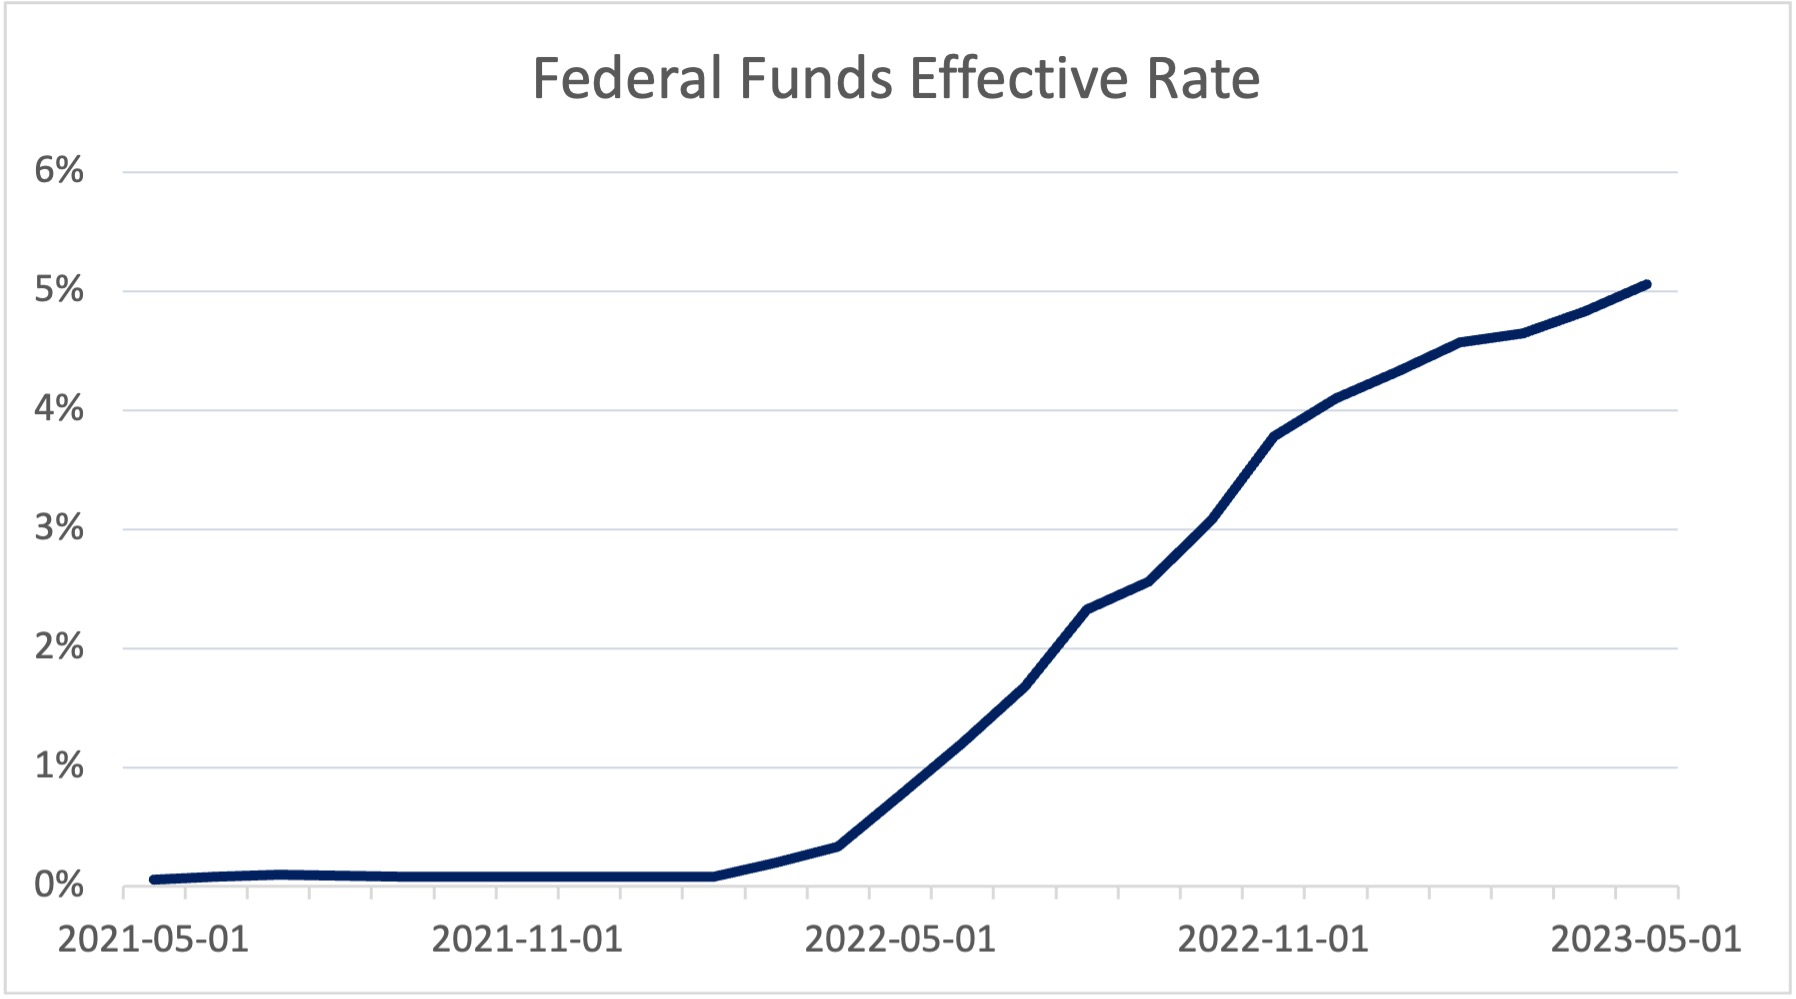
\includegraphics[height=5.5cm]
    {assets/FEDRATES.jpg}
\end{center}

Another assumption and oversimplification made in these computations, analyzing portfolio performance, is the omission of dividend payments from the equities' returns. Additionally, considering that some of the computed portfolios have significant allocations to energy sector stocks, it's plausible to argue that investors might be predominantly interested in these stocks for their returns in the form of dividends.

\begin{center}
    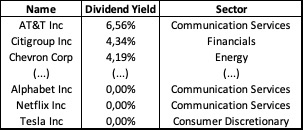
\includegraphics[height=3cm]
    {assets/Divid.jpg}
\end{center}

\subsection*{Performance Evaluation and Discussion}

Using now the new data but with the previously computed allocation we can properly test how the portfolios would have performed on the market in the following year 12/05/2022-12/05/2023.

\begin{center}
    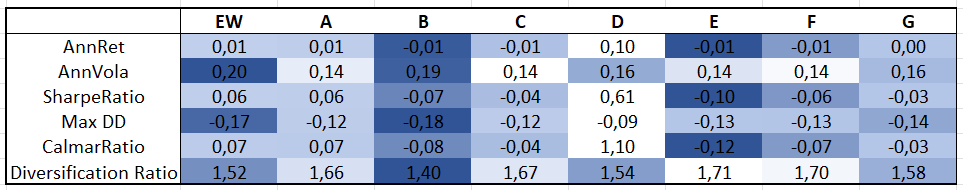
\includegraphics[height=2.5cm]
    {assets/Blue3.png}
\end{center}

\begin{center}
    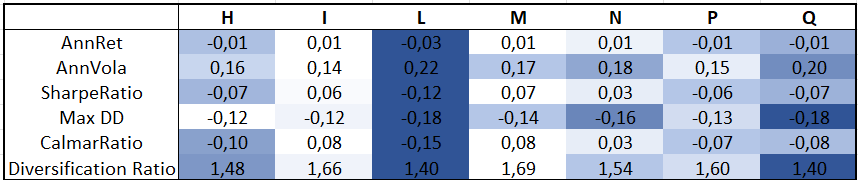
\includegraphics[height=2.5cm]
    {assets/Blue4.png}
\end{center}

It's immediately clear that the performance of all our portfolios drops sharply. This could be explained by various factors, the main being the static nature of the weights computed with old data and the change in market behaviour and conditions yearly. Metrics such as the Sharpe Ratio are dependent on the data it has been computed on, in our case it is relative to the rolling year 11/05/2021 to 11/05/2022, that has very little correlation to performance in the following year. This is even more relevant since the socio-economic conditions changed drastically from 2021 to 2023 with the end of the expansionary measures and stimuli, and the increase in interest rates to combat inflation.
\\
The best performing portfolio overall is Portfolio D and this mostly comes down to two main factors.
Firstly, portfolio D maximizes the Sharpe Ratio, which grants higher returns, and, secondly, it satisfies some sector constraints that actually preserved it from the paradigm change that happened between 2021 and 2023.
Indeed, the portfolio outperforms even the standard constrained equivalent.
\\
On the opposite end, the worst performing portfolio overall is portfolio L.
This is probably due to the fact that the Black-Litterman approach views were not realized in the following year with respect to the maximization of the Sharpe ratio.
\\
The diversification rate does change significantly, in other words, the correlation between different equities changes significantly from one year to the next. This is probably a symptom the paradigm change observed in the markets in 2023.
To further support this hypothesis, we can observe that portfolio P, which was comprised of stocks that drove the market in 2021-2022, performs rather poorly in part B. \\
In conclusion, we can observe that almost all portfolios do not outperform the trivial equally weighted portfolio with respect to the Annualized Return. In other words, the information gathered on the market in part A does not inform a good investment in part B due to the change in market behaviour.
In the picture below we can see the Equity of the most interesting portfolios of Part A.

\begin{center}
    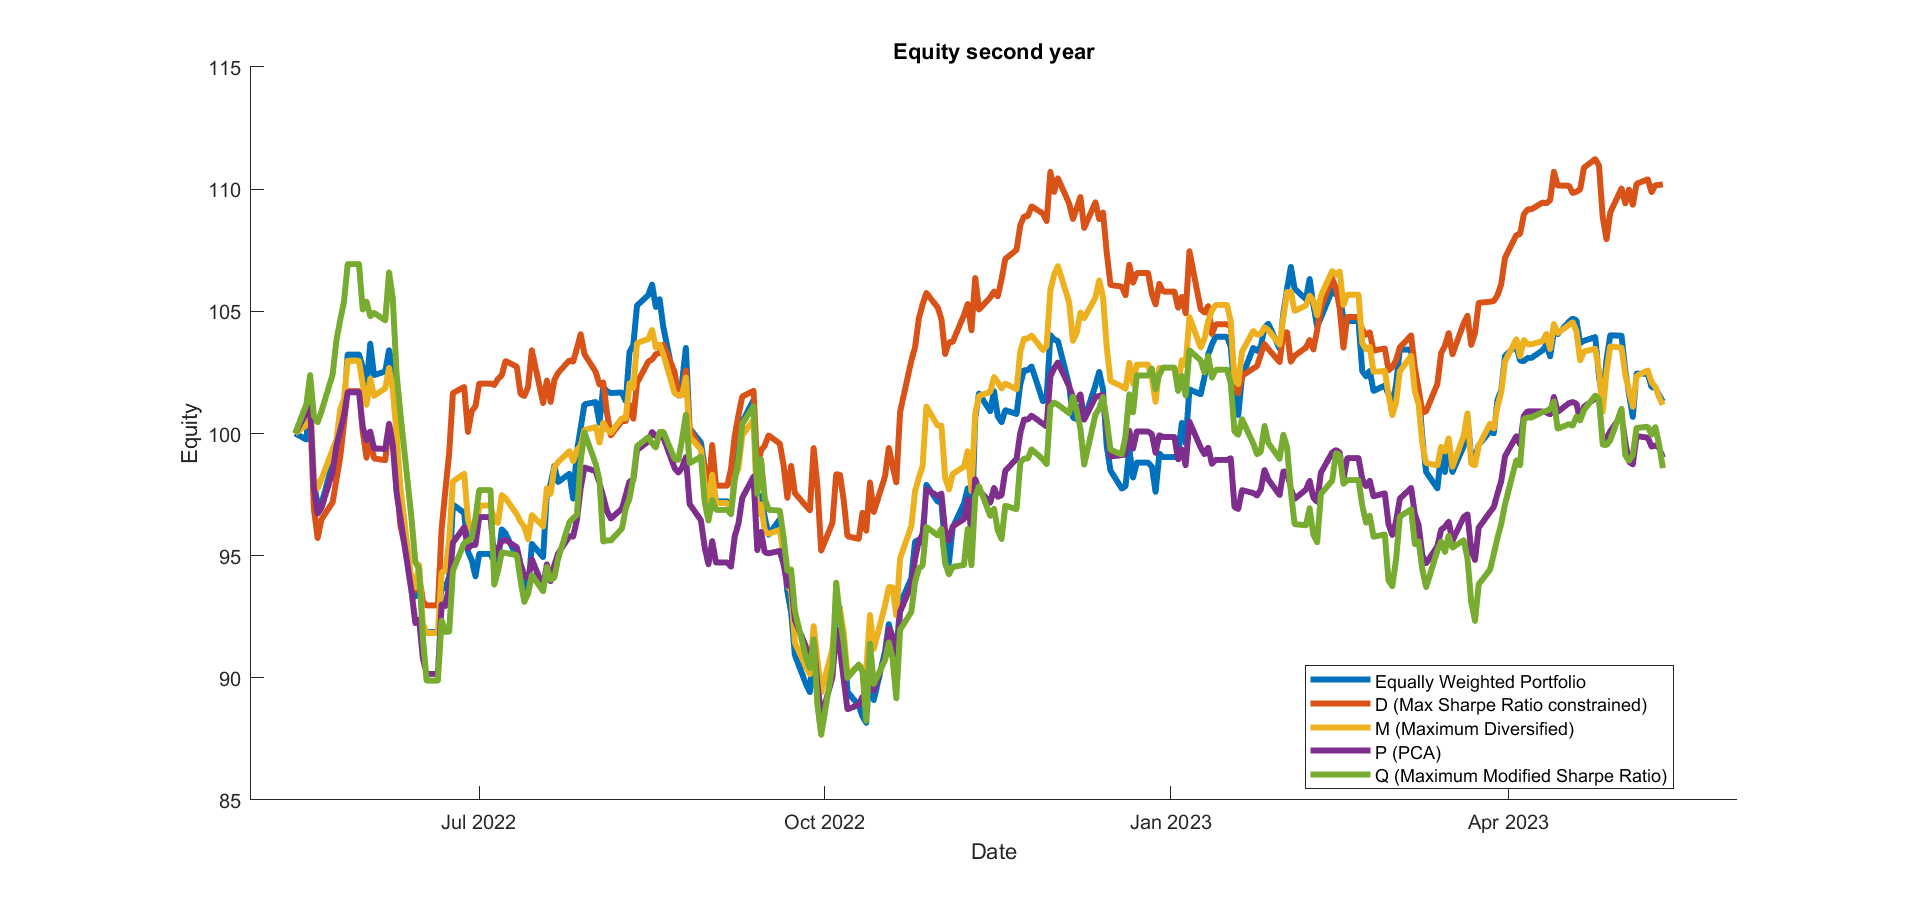
\includegraphics[height=7cm]
    {assets/Equity2.png}
\end{center}


\end{document}

